\documentclass[letterpaper,twocolumn,10pt]{article}
\usepackage{usenix2019_v3}
\usepackage{amsmath}
\usepackage{booktabs}
\usepackage{array}
\usepackage{graphicx}
\usepackage{tikz}
\usepackage{pgfplots}
\usetikzlibrary{arrows.meta,positioning}
\pgfplotsset{compat=1.18}
\pagestyle{plain}
\hypersetup{pdfauthor={AI-generated working draft},
	pdftitle={Decoupling Workload Admission from Policy Materialization in Kubernetes},
	pdfsubject={Non-submission writing exercise}}
\newcommand{\sys}{\textsc{KNP}}

\title{\Large\bf Decoupling Workload Admission from\\
Policy Materialization in Kubernetes}
\author{AI-generated working draft for author discussion\\
Non-submission exercise; Traditional Research framing}
\date{}

\begin{document}
\maketitle
\noindent\textbf{Editorial notice.} This is an AI-generated writing exercise,
not a submission or text attributed to Antonio Ojea. It develops the proposed
research argument using the available evidence. Implementation inspection,
archived measurements, operator-reported outcomes, and analytical predictions
are distinguished throughout. The evaluation is incomplete.

\begin{abstract}
Network policy enforcement must keep pace with the creation and replacement
of the workloads it protects. Indexed kernel lookups and incremental datapath
updates improve packet processing, but they do not by themselves remove the
cost of translating changing workload metadata into distributed enforcement
state. We examine a different placement of that work: evaluate Kubernetes
policy semantics in userspace when communication is attempted, and reuse
accepted decisions through the kernel's connection tracker. The
kube-network-policies implementation combines NFQUEUE-based admission with
nftables packet steering; runtime integration provides local Pod metadata
without waiting for its asynchronous publication through the Kubernetes API.
We characterize the design using source inspection and archived experiments
targeting 35,000 Pods on a reported 720-worker testbed. Completed Cilium
identity sweeps retain low post-scheduling latency and flat worker CPU
(0.51--0.63 mean cores) across 7 to 35,000 intended identities, while the
35,000-ReplicaSet tiers halve achieved Pod throughput (170 versus
280--330 Pods/s) and a dense-mesh tier was excluded because its estimated
per-endpoint permission state exceeded the stated map capacity. An earlier
Cilium release stranded Pods at 700 identities, and a separate direct-burst
experiment stranded 5,694 Pods. These observations motivate distinguishing
latency, throughput, capacity, and admission failure, rather than treating
identity cardinality as a single scaling variable. We identify the conditions
under which deferred evaluation reduces eager policy state and evaluate a
kube-network-policies bidirectional mesh sweep that matches Cilium's at
three ReplicaSet-paced tiers (7, 700, and 3,500 identities) and adds an
unmatched 35,000-identity raw-Pod tier. Because every sandbox blocks in an
init container until a permitted TCP connection to a gateway succeeds, the
reported post-scheduling latency bounds time to first permitted
communication, including cross-node metadata convergence. At 700 and
3,500 identities kube-network-policies reaches 5.33 s and 2.79 s P99,
within 2.4 s of Cilium at 2.5--3$\times$ lower achieved Pod throughput;
at 7 identities with 5,000 Pods per ReplicaSet its P99 is 151 s against
Cilium's 6.8 s under the same generator; and the 35,000 raw-Pod tier, which
Cilium's producer excluded analytically, completes with all Pods Running
but a 421 s P99 whose cause the artifacts do not isolate. We analyze the
connection-processing and fail-open trade-offs of deferred evaluation and
enumerate the measurements still needed to complete the comparison.
\end{abstract}

\section{Introduction}
The unit of isolation in a container cluster is also a unit of change.
A service scales out, a job completes, or a sandbox is replaced; its network
permissions must follow that lifecycle. For long-lived services, much of this
work can be amortized over hours of communication. Short-lived workloads
offer less time to recover their setup cost. Agent execution environments
provide one motivation for this regime, alongside batch jobs and serverless
functions, although the experiments considered here are synthetic sandbox
workloads rather than traces of deployed agents.

Kubernetes makes the problem more subtle than installing a firewall rule
for a new address. NetworkPolicies describe permitted relationships through
Pod labels, namespace labels, ports, and address ranges. Addresses and
placement change independently of this intent. An implementation must join
policy with current workload metadata, establish isolation at the appropriate
point in the workload lifecycle, and handle updates while packets continue
to arrive. A fast packet lookup is necessary in many settings, but it is
not a complete answer to these coordination costs.

Successive enforcement mechanisms have addressed different parts of this
problem. Linear chains give way to indexed sets and maps. Programmable
datapaths separate packet-processing code from mutable state. Distributed
network virtualization compiles logical intent into local actions and
caches expensive decisions. These mechanisms are complementary, not a
sequence of obsolete technologies. In particular, nftables supports
incremental updates, and userspace miss handling followed by kernel caching
is central to Open vSwitch~\cite{winship2025nftables,pfaff2015ovs}. The next
question is therefore not which kernel mechanism is newest. It is which
work must occur before a workload can communicate, and how much of that
work must be repeated elsewhere in the cluster.

This paper examines \emph{deferred semantic evaluation} for Kubernetes
network policy. In kube-network-policies, hereafter \sys{}, a node agent
receives packets selected by nftables through NFQUEUE, resolves the relevant
metadata, and evaluates the policy in userspace. An accepted verdict records
an acceptance label in conntrack. Eligible subsequent traffic follows the
kernel path without repeating the semantic evaluation. The engine does not
require a separate policy-specific distributed security-identity allocator
or a per-endpoint expansion of every permitted peer identity. It still
requires metadata distribution, packet steering, and per-connection state.

The design trades eager permission materialization for work at attempted
communication. If a policy permits a large peer set but a workload contacts
only a few peers, maintaining every possible relationship may be unnecessary.
Conversely, a workload creating many short connections can make the queue
and userspace evaluator the bottleneck. Denied traffic is especially
important: repeatedly rejected attempts do not benefit from the accepted
connection cache. The research question is whether this tradeoff is favorable
for high-churn clusters, not whether userspace processing is universally
faster than in-kernel processing.

Local startup observation is a second part of the design. Kubernetes
publishes a Pod's address asynchronously. A policy agent relying exclusively
on that publication can learn the address after a container has started
using it, or after a lifecycle hook has begun waiting for network access.
The longstanding issue documented in Kubernetes issue 85966 illustrates
this dependency~\cite{k8s85966}. Node Resource Interface (NRI) integration
obtains local sandbox metadata through the runtime, removing that particular
round trip from local address discovery. It does not eliminate namespace
or policy convergence, nor establish a cluster-wide startup barrier.

Our evidence distinguishes five observations. First, the completed
Cilium identity sweeps do not show an increasing post-scheduling latency
curve: the intended 35,000-identity open-gateway configuration has a
1.99-second P99, and mean worker CPU stays within 0.51--0.63 cores across
all tiers. Second, the 35,000-ReplicaSet tiers reduce achieved Phase-1
throughput from roughly 280--330 to 170 Pods/s and raise cluster-scoped
Pod LIST P99 latency from 14--19 s to 28.8 s; the controller fan-out, not
the datapath, is the visible bottleneck there. Third, under the benchmark's
per-endpoint expansion model, a bidirectional mesh with 35,000 identities
requires approximately 70,000 peer-policy entries per endpoint. The
experiment producer excluded that tier on predicted capacity grounds; it was
not executed on Cilium. Fourth, two Cilium admission failures are recorded: an archived
Cilium v1.18.6 run stranded 19 of 35,000 Pods at 700 identities, attributed
to a policy-cache race fixed in v1.20.0~\cite{cilium7515}, and a
v1.20.1 raw-Pod burst aborted with 29,306 Pods Running and 5,694 stranded,
attributed to endpoint throttling and cumulative identity allocation.
Fifth, a \sys{} bidirectional mesh sweep matched to Cilium's at the three
ReplicaSet-paced tiers shows no increase in post-scheduling P99 from 700
to 3,500 identities (5.33 s to 2.79 s), but a 151 s P99 at the
5,000-Pods-per-ReplicaSet tier where Cilium records 6.8 s, and an
unmatched 35,000-identity raw-Pod tier that completes with all Pods
Running at a 421 s P99. The \sys{} runs also achieved 2.5--3$\times$
lower Pod throughput than Cilium's, so the sweep does not by itself
separate identity cost from generator pacing. None
of these observations should be substituted for another.

The paper develops three contributions at different levels of evidence.
It describes a working enforcement decomposition based on existing Linux
mechanisms, including a security analysis of its fail-open and
unknown-peer behavior; presents a conditional model of eager permission
state versus connection-driven work; and analyzes an archived
large-cluster benchmark collection across both Cilium and \sys{}, including
the newly executed \sys{} mesh sweep. Section~\ref{sec:gaps}
enumerates what the artifacts still do not contain: the \sys{} sweep has
one trial per tier, its agent-level metrics returned no samples, its
35,000-identity tier has no Cilium counterpart under the same policy, and
no denied-traffic or overload measurement exists. Making those limits
explicit lets the evaluation test the design rather than assuming its
conclusion.

\section{Background and Problem}
\label{sec:background}
\subsection{Policy Semantics and Workload Lifecycle}
Kubernetes NetworkPolicy isolates ingress and egress independently. Within
a direction, the permissions of applicable standard NetworkPolicies combine
additively. A connection between two isolated Pods must satisfy the source's
egress policy and the destination's ingress policy; reply traffic for an
allowed connection is implicitly permitted~\cite{k8snetworkpolicy}. This
connection-oriented interpretation makes reuse of admission decisions
natural, although it does not require any particular conntrack implementation.

Policy creation and workload creation have different synchronization
requirements. A newly submitted policy is handled asynchronously, and the
API does not expose a general enforcement-completion barrier. Once a plugin
has handled a policy, newly created selected Pods must be isolated before
their containers start. Allow permissions may converge later. Thus a system
can preserve isolation while temporarily delaying legitimate communication.
Safety and availability must be measured separately; a fast transition to
\texttt{Running} is not proof of either.

We distinguish four quantities that are often conflated: live endpoints,
distinct policy-relevant label sets, allocated numeric security identities,
and materialized datapath entries. Several Pods can share an identity.
One identity can contribute permissions to many endpoint maps. Allocations
not yet reclaimed can outlive their original workload. The number of
permitted relationships also differs from the number of active connections.
The resulting scaling dimensions are related but not interchangeable.

\subsection{Placement and Timing of Enforcement Work}
\paragraph{Chains, sets, and incremental updates.}
An ordered chain can perform work proportional to the number of rules
visited. This does not imply that every iptables deployment performs a
linear address lookup: ipset supplies indexed membership, while nftables
integrates sets and verdict maps. Sutter's 2017 measurements demonstrate
the importance of this representation choice, with both nftables sets and
iptables with ipset maintaining throughput across the tested
ranges~\cite{sutter2017nftables}. More recent Kubernetes work describes
incremental nftables updates that scale with changed Service state rather
than the full Service ruleset~\cite{winship2025nftables}. Service proxying
is not NetworkPolicy, but it demonstrates why lookup and update mechanisms
must be discussed independently.

\paragraph{Virtual networking and reactive caches.}
NVP and Open vSwitch address the translation from logical networks to
physical forwarding~\cite{koponen2014nvp,pfaff2015ovs}. OVS caches
flow-processing results and sends misses to userspace; its evolution
illustrates both the value and the cost of reactive processing. OVN also
supports stateful ACLs, including \texttt{allow-related} actions backed by
connection tracking~\cite{ovnacl}. A comparison that describes these
systems as inherently stateless would miss the closest precedents for
our design.

\paragraph{Programmable datapaths and identities.}
eBPF maps permit userspace to update keyed state without replacing the
packet-processing program~\cite{linuxbpfmaps}. Cilium uses label-derived
security identities to represent workloads~\cite{ciliumidentities}.
Identity sharing can avoid repeating work for equivalent workloads, but
distinct labels and broad selectors can still create allocation,
distribution, and materialization work. These are properties of an
architecture and configuration, not intrinsic restrictions of eBPF. The
size of a numeric identity space and the capacity of a policy map are
different limits.

\paragraph{Problem statement.}
We ask whether policy enforcement can retain the established kernel
forwarding path while avoiding eager expansion of all permitted peers
at each endpoint. A useful solution must explain where the displaced work
goes, how local admission obtains sufficiently fresh metadata, and how
existing decisions interact with changing policy. Packet throughput alone
cannot answer these questions.

\section{Design}
\label{sec:design}
\subsection{Connection Admission and Cached Decisions}
\sys{} separates policy interpretation from packet steering. Kubernetes
objects supply policy intent and workload metadata to the node agent.
nftables identifies traffic requiring a decision and sends it to NFQUEUE.
The callback parses packet headers, invokes the userspace evaluator, and
returns an accept or drop verdict. For an accepted decision it supplies a
conntrack label, which the kernel rules can subsequently recognize.
Figure~\ref{fig:architecture} illustrates the separation.

\begin{figure}[t]
\centering
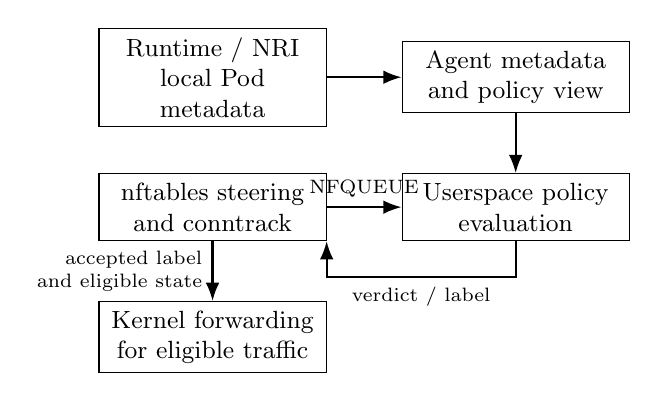
\begin{tikzpicture}[
	box/.style={draw,align=center,text width=2.65cm,minimum height=0.85cm,font=\small},
	flow/.style={-{Latex},thick},font=\scriptsize]
\node[box] (runtime) at (0,0) {Runtime / NRI\\local Pod metadata};
\node[box] (metadata) at (3.85,0) {Agent metadata\\and policy view};
\node[box] (kernel) at (0,-1.65) {nftables steering\\and conntrack};
\node[box] (evaluate) at (3.85,-1.65) {Userspace policy\\evaluation};
\node[box] (forward) at (0,-3.3) {Kernel forwarding\\for eligible traffic};
\draw[flow] (runtime) -- (metadata);
\draw[flow] (metadata) -- (evaluate);
\draw[flow] (kernel.east) -- node[above]{NFQUEUE} (evaluate.west);
\draw[flow] (evaluate.south) -- ++(0,-0.45) -| node[pos=0.25,below]{verdict / label} (kernel.south east);
\draw[flow] (kernel.south) -- node[left,align=right]{accepted label\\and eligible state} (forward.north);
\end{tikzpicture}
\caption{Enforcement decomposition, omitting protocol and host-traffic
exceptions. Kubernetes watches also feed the agent's policy and metadata
view. NRI supplies local observations, not remote policy synchronization.}
\label{fig:architecture}
\end{figure}

The cached decision is connection state, not a precomputed table of every
allowed peer. In the inspected forwarding path, the bypass rule requires
both the acceptance label and an established or related conntrack state.
Uncached managed traffic is queued. Consequently, ``first-packet
evaluation'' is a useful intuition but not an exact accounting rule:
several initial packets, retransmissions, or protocol-specific transitions
can reach userspace before the bypass condition holds. Denied packets
do not acquire the accepted-decision cache entry.

nftables remains part of the implementation. It maintains steering rules
and managed-address sets, rather than executing Kubernetes label selectors
as a shared kernel policy table. Avoiding peer-permission expansion does
not imply eliminating every local rule update. Changes to managed
endpoints or enforcement scope can still require steering reconciliation.
The policy evaluator's own metadata indexes and selector processing also
consume CPU and memory.

The decision is local once the required metadata has arrived: the packet
path does not allocate a new distributed numeric identity for the attempted
connection. This is a receive-driven policy metadata path, not a claim
that the entire network control plane is read-only. The runtime, address
management, routing, and Kubernetes controllers continue to update their
own state. Remote endpoint metadata must still reach the enforcing node.

\subsection{Runtime Metadata and Startup Isolation}
Consider the dependency chain when a node learns its own Pod's IP only
through Kubernetes status. The runtime creates the sandbox and configures
networking; the kubelet publishes status to the API server; a watch event
reaches the policy agent. Container or lifecycle-hook activity can occur
before the last step. If that activity waits for network permissions that
depend on the status update, observation delay becomes application delay.
Issue 85966 records precisely this problem for policy-only
networking~\cite{k8s85966}.

The NRI resolver populates a local IP-to-Pod metadata cache in its
\texttt{RunPodSandbox} callback. It uses addresses supplied by the runtime
API and can fall back to inspection of the sandbox network namespace.
This places local observation at the runtime boundary instead of behind
the kubelet--API-server--watch round trip. Subject to the runtime's callback
ordering and successful metadata acquisition, it makes the local address
available before application-container execution requires it.

There are two limits to this improvement. First, obtaining metadata is
not the same as installing effective isolation. The integration must
ensure the steering path cannot bypass policy before protection applies.
Second, namespace labels, policy objects, and remote peers can still be
asynchronous. A claim of zero startup latency would therefore be incorrect.
The narrower claim is removal of a specific asynchronous dependency in
local address discovery; an NRI-on/off timing and connectivity experiment
is needed to quantify its benefit.

\subsection{Policy Changes and Failure Semantics}
Caching makes policy changes part of the correctness argument. Standard
NetworkPolicy leaves the effect of updates on already established
connections implementation-defined~\cite{k8snetworkpolicy}. \sys{}
also provides a strict mode that scans conntrack entries, reevaluates
supported flows, and clears the acceptance label where current policy
no longer permits communication. Subsequent processing can then revisit
the decision. This introduces work proportional to the flows inspected
and the complexity of reevaluation; it is not an instantaneous revocation
mechanism. The enforcement delay must include event delivery, scan
scheduling, scan execution, and subsequent packet handling.

Failure policy must be equally explicit. NFQUEUE can drop packets on
queue overflow or accept them when configured fail-open~\cite{nfqueueapi}.
The inspected command-line interface defaults to fail-open, and the
dataplane sets the queue's bypass flag whenever fail-open is enabled,
with a maximum queue length of 1,024 packets. Two facts about the cached
path make this a security-relevant default rather than an operational
detail. Denied packets never acquire the acceptance label, so every
retried forbidden connection attempt re-enters the queue; and a workload
that can emit uncached packets faster than the agent returns verdicts
fills the queue. Under fail-open, the overflow is then \emph{accepted}
by the kernel without evaluation. A tenant that is permitted to run code
in the cluster can therefore attempt to convert denied traffic into a
bypass by saturating its node's agent, and its own denied attempts are
the cheapest saturating traffic. The inspected implementation has no
per-source rate limit or denied-flow negative cache that would blunt this
amplification; the only countermeasure is \texttt{--fail-open=false},
which converts overload into loss of connectivity for every managed Pod
on the node. Quantifying the overload point is therefore part of the
safety argument, not only of the performance argument. The benchmark
manifest in the repository sets \texttt{--nfqueue-id} but not
\texttt{--fail-open}, so the archived \sys{} runs executed with the
fail-open default.

Unknown peers have a different failure mode. When the evaluator cannot
resolve a remote source or destination address to Pod metadata, the
inspected selector matching treats a \texttt{nil} peer as matching only
\texttt{ipBlock} rules; Pod and namespace selectors never match it. Under
a default-deny policy the packet is dropped. This is fail-closed at the
policy level, and it is the correct isolation behavior, but it means a
permitted connection from a freshly created remote Pod is denied until
the destination node learns the source's metadata. NRI removes this
delay only for \emph{local} Pods. For remote peers the agent still
depends on API-server watch delivery, or on the IPTracker distribution
tier of Section~\ref{sec:iptracker}, and the observed delay is an
availability cost. The benchmark's startup gate exercises exactly this
path: a new sandbox's first connection is admitted at the gateway node
only after that node has learned the sandbox's address, so the
\texttt{schedule\_to\_run} latencies of Section~\ref{sec:evaluation}
contain this convergence time rather than exclude it.

Further, the inspected implementation logs an initial nftables
synchronization error without blocking startup, and its fail-closed
graceful-shutdown path removes its nftables rules. Those transitions
require a deployment-level isolation contract or implementation changes
before claiming protection throughout the lifecycle.

We therefore state the desired safety property conditionally. For a
policy already handled by an agent, a new selected workload must not
send or receive forbidden traffic before enforcement takes effect.
An allowed connection may be delayed by missing information; such delay
must not be confused with an isolation violation. The current benchmark
collection does not establish this property. A complete validation must
exercise missing metadata, label changes, IP reuse, failures, and init
containers as well as steady-state allow/deny behavior.

The intended trust boundary includes the node kernel, runtime, policy
agent, and the CNI's endpoint/address binding. Untrusted workloads must
not be able to impersonate a peer by spoofing its address. Privileged
workloads, host networking, and enforcement around address translation
need explicit scope. NFQUEUE and NRI do not independently establish
those assumptions.

\section{Where the Scaling Cost Moves}
\label{sec:model}
Let $I$ denote selected peer identities, $P_{\ell}$ local endpoints,
$d$ the number of materialized directions, and $F_{\ell}$ locally tracked
active connections. In an eager representation with a distinct entry
per peer identity and direction at every endpoint, the peer-policy
contribution is
\begin{equation}
E_{\mathrm{endpoint}} \approx dI,\qquad
E_{\mathrm{node}} \approx dIP_{\ell}.
\label{eq:materialization}
\end{equation}
This is a conditional representation model, not a lower bound on all
policy implementations. Sharing, wildcarding, aggregation, or another
representation can change it. Additional policy rules contribute further
entries. Entry counts are also not byte counts: data-structure overhead,
preallocation, and sharing must be measured separately.

Under the same assumptions, a new identity selected by every local
endpoint can induce approximately $dP_{\ell}$ local entry updates. For
a rate $\lambda_I$ of such new identities, the corresponding update
demand is approximately $dP_{\ell}\lambda_I$. Identity dissemination,
selector recomputation, and endpoint regeneration are separate costs;
none is measured by this expression. With a shared identity, many Pod
replacements may leave this demand nearly unchanged. Fresh-identity
churn is consequently a different workload from Pod churn.

Deferred evaluation removes this particular eager cross-product, but
retains metadata, steering state, and conntrack. A useful accounting is
\begin{equation}
M_{\mathrm{deferred}} = M_{\mathrm{metadata}} +
M_{\mathrm{steering}} + M_{\mathrm{conntrack}}(F_{\ell}).
\end{equation}
It is not a proof that total memory is smaller than in an identity-based
engine: both may already maintain conntrack, and the userspace metadata
representation can dominate. The avoided term is materialized permission
state; the comparison must account for all other state on both sides.

Let $\lambda_q$ be the actual queued-packet rate and $\mu$ the aggregate
sustainable verdict-processing rate. Avoiding sustained queue growth
requires, as a first-order condition,
\begin{equation}
\rho = \lambda_q/\mu < 1.
\end{equation}
Burstiness, shared CPU, and scheduling can produce tail latency and drops
even below this average-load condition. Queue demand includes denied
attempts and repeated initial packets, not just successfully established
connections. The only measurement of $\mu$ available to us is the
repository's own three-node ApacheBench microbenchmark~\cite{knptesting}:
10,000 non-keepalive HTTP requests at concurrency 1,000 completed at
2,317 requests/s with a 5-ms median and a 3,080-ms P99 dominated by
connect time, while the kernel logged \texttt{nf\_conntrack: table
full} at the default 262,144-entry limit. The accompanying Prometheus
charts show per-node queued-packet peaks near 8,000 packets/s and
callback durations with medians of 80--120 $\mu$s and P99s of
170--630 $\mu$s. Hardware, kernel, and agent version are not recorded,
and conntrack exhaustion confounds the tail, so we treat these as an
order-of-magnitude bound on a single node's verdict capacity, not as a
characterization of $\mu$. The 720-node startup reports do not
establish $\lambda_q$ at all.

The favorable regime is thus not simply ``many identities.'' It is a
large or rapidly changing set of possible permissions relative to the
communication actually attempted, with sufficient admission-processing
capacity. A dense \emph{permission} graph can still produce sparse traffic.
A dense \emph{active connection} graph, frequent revocation, or sustained
denied traffic can remove that advantage. This distinction supplies
testable hypotheses without assuming a particular technology must win.

\section{Implementation}
\label{sec:implementation}
The inspected implementation is the Go-based kube-network-policies
repository at revision \texttt{9984dcd}. Its dataplane controller uses
nftables through netlink and the NFQUEUE interface for packet delivery
and verdicts. The queue is configured with a maximum length of 1,024,
a copy length of 128 bytes, GSO support, and a 100-ms write timeout.
These are implementation settings, not measured service rates or tail
latency bounds. Limiting the copy to headers avoids copying whole
payloads for policy decisions, but requires checking parser behavior
for options, extension headers, fragmentation, and truncation.

The callback resolves policy through an evaluator interface and emits
an acceptance conntrack label with the verdict. Metrics record callback
processing time, protocol/family-specific verdict counts, queue occupancy,
and drop counters. Callback time does not include every component of
kernel-to-userspace waiting time, so it cannot alone represent
application-visible connection setup. The benchmark harness did not
scrape these agent metrics: its Prometheus queries cover node and
kubelet CPU only, and a \texttt{kindnetd} CPU query in the saved
configuration returned no samples. The implementation also has
host-traffic and protocol exceptions; the conceptual cached path in
Figure~\ref{fig:architecture} is not a complete description of all hooks.

The repository builds several flavors of the agent. The standard flavor
queues only traffic to or from local Pods selected by some policy,
maintained as nftables sets of managed addresses. The IPTracker flavor
inspected at the same revision instead reports \emph{divert-all}: it
queues every forwarded packet not already bypassed by conntrack,
because it watches only NetworkPolicy objects and has no Pod informer
from which to enumerate the local Pods a policy selects. The two flavors
therefore have different $\lambda_q$ for the same workload, and the
queue-overload analysis of Section~\ref{sec:design} applies to a larger
traffic fraction in the IPTracker flavor.

The NRI resolver is an alternate source of local Pod metadata, not a
replacement for every informer. Its callbacks add and remove local
records; namespace information can still come from the API-derived
view. This modularity permits policy logic to evolve as ordinary
userspace code while the steering mechanism remains relatively stable.
We regard reduced feature-development coupling as an architectural
property, not a measured productivity result. New policy features may
still require additional metadata, hook coverage, or cache invalidation.

An experimental distinction is essential: \sys{} names the inspected
policy engine, while the benchmark directories label complete networking
configurations as \emph{Kindnet} or \emph{Cilium}. Those configurations
include networking and runtime components beyond policy evaluation.
The benchmark repository pins Cilium v1.20.1 in its cluster specification
and a \texttt{kube-network-policies:v1.1.0} image in its standalone
install manifest, but the \sys{} cluster was created with the Kindnet
CNI's bundled policy agent, patched to \texttt{kindnet:v1.0.1} with an
NRI socket mount; which policy binary and flags were effective in each
Kindnet run is not recorded in the artifacts. We therefore do not
attribute their latency differences solely to the code described here.

\section{Evaluation}
\label{sec:evaluation}
\subsection{Methodology and Provenance}
We analyze archived ClusterLoader2 artifacts rather than execute a new
cluster experiment. The repository describes a testbed with 720
\texttt{n2-standard-4} workers, a \texttt{c4-standard-96} control-plane
node, and a target of 35,000 concurrent Pods. The runtime configuration
is reported as containerd 2.2.4 with runc 1.3.5. These are environment
descriptions, not a reconstructed per-run inventory; topology and binary
provenance must be confirmed before pooling runs from different dates.

The extraction at benchmark revision \texttt{e8af592} inventories 1,809
artifact files and parses 1,285 JSON files, recovering 55 startup reports.
Including diagnostic-only directories yields 62 attempts, seven without
a startup report. Later revisions \texttt{0442dce} and \texttt{f998224}
add descriptions of the raw-Pod abort and mesh-tier exclusion, respectively.
Those records are used as documented outcomes, not as replacement timing
samples. Appendix~\ref{sec:provenance} identifies the relative source paths.

We distinguish \texttt{create\_to\_schedule},
\texttt{schedule\_to\_run}, and total \texttt{pod\_startup}.
The middle quantity includes runtime and container work, and in this
harness it also includes a connectivity gate: every sandbox Pod template
carries a \texttt{wait-for-gateway} init container that loops
\texttt{nc -z} against the gateway Service until a TCP connection
succeeds. The sandbox is egress-isolated and the gateway is
ingress-isolated by the deployed policies, so a Pod reaches
\texttt{Running} only after one \emph{permitted} connection has been
admitted by both the source node's egress evaluation and the gateway
node's ingress evaluation. \texttt{schedule\_to\_run} is therefore an
upper bound on time to first permitted communication for the
sandbox-to-gateway path, and it includes propagation of the new Pod's
address to the gateway node. It does not test sandbox-to-sandbox
permissions, exercises no forbidden path, and under \sys{}'s fail-open
default would also pass if the queue overflowed. The init container logs
its own wait as \texttt{Latency: N ms}; those per-Pod values were not
collected. Component percentiles cannot be added to reconstruct a total
percentile. Likewise, a configured object-operation QPS is not necessarily
achieved Pod throughput: a ReplicaSet operation can create multiple Pods.

Negative enforcement was checked once per cluster, not per run:
\path{scripts/verify-netpol.sh} creates a client and server, confirms
connectivity, applies a default-deny ingress policy and confirms the
request is blocked, then applies an explicit allow and confirms it
succeeds. Its output is not archived, and it ran on an idle cluster
before the sweeps. The benchmark therefore establishes positive
enforcement at scale and negative enforcement only as a quiescent smoke
test.

Saved configurations take precedence over the current generator. The
September identity sweeps vary Pods per ReplicaSet along with intended
identity cardinality, use the default scheduler, and replace 5,000 Pods
per churn round. Five rounds within a run are not five independent trials.
The number of allocated Cilium identities must also be distinguished
from the generator's intended label cardinality. We retain per-run
percentiles and completion indicators, rather than constructing CDFs
or confidence intervals from summary quantiles.

\subsection{Workload Admission and Identity Turnover}
Table~\ref{tab:identity} reports completed September identity tiers
across Cilium (open gateway, hub-and-spoke, and bidirectional mesh) and
\sys{} (bidirectional mesh). All target 35,000 Pods at 500 QPS.
Within the ReplicaSet-paced tiers from 700 identities upward, increasing
intended identities does not produce an increasing post-scheduling tail
for either engine. In Cilium's open-gateway case, P99 decreases from
5.930 s to 1.990 s between the endpoint tiers (hub-and-spoke: 6.370 s to
2.033 s). In the bidirectional mesh, \sys{} P99 falls from 5.331 s at 700
identities to 2.791 s at 3,500 (P50: 3.273 s and 2.234 s), within 2.4 s
and 0.5 s of Cilium's 2.934 s and 2.279 s on the same generator.

The two remaining \sys{} tiers are not flat. At 7 identities with 5,000
Pods per ReplicaSet, \sys{} records 38.946 s P50 / 151.479 s P99 where
Cilium records 1.41 s / 6.767 s under the identical configuration: a
22$\times$ gap in P99 that the artifacts do not explain. It is consistent
with the July Kindnet baseline (57 s P99) and tuned run (9.7 s
post-scheduling, 95.8 s total) at the same 5,000-Pods-per-ReplicaSet
shape, so the large-ReplicaSet burst, not identity count, is where the
\sys{} configuration degrades. The 35,000-identity tier was run as
35,000 raw Pods under the mesh policy; it has no Cilium counterpart, since
Cilium's producer excluded the mesh tier analytically and Cilium's only
raw-Pod run used the hub-and-spoke policy and aborted. \sys{} completed
it with all 35,000 Pods Running and no stranded Pods, at 120.003 s P50 /
421.410 s P99 post-scheduling and 139.6 s / 499.9 s end-to-end; the
harness recorded two failures against its 5-minute P90 startup SLO.
\texttt{create\_to\_schedule} reached 106.7 s P99, so scheduling itself
took well over a minute for the tail. Candidate causes for the
post-scheduling tail include serialized sandbox creation in kubelet
(about 49 Pods arrive per node), convergence of 35,000 new Pod addresses
to the gateway nodes before their init containers can be admitted, and
API-server watch latency; the kubelet CNI-latency and agent queries
returned no samples, so the artifacts do not separate them.

\begin{table}[t]
\centering
\small
\setlength{\tabcolsep}{2.5pt}
\begin{tabular}{rrrrrr}
\toprule
Intended & Pods/ & \multicolumn{3}{c}{Cilium P99 (s)} & \sys{}\\
identities & RS & GW & Spoke & Mesh & Mesh P99\\
\midrule
7 & 5,000 & 5.930 & 6.370 & 6.767 & 151.479\\
700 & 50 & 5.416 & 4.759 & 2.934 & 5.331\\
3,500 & 10 & 4.685 & 4.899 & 2.279 & 2.791\\
35,000 & 1 & 1.990 & 2.033 & Excl. & ---\\
35,000 & Raw & --- & Abort$^{\dagger}$ & --- & 421.410$^{*}$\\
\bottomrule
\end{tabular}
\caption{Per-run archived schedule-to-run P99. All ReplicaSet-paced
suites have zero JUnit failures. $^{\dagger}$Cilium raw-Pod hub-and-spoke
run aborted at 29,306 Running / 5,694 stranded. $^{*}$\sys{} raw-Pod mesh
run: 35,000 Running, 0 stranded, two JUnit failures against the 5-minute
P90 startup SLO (observed 357.7 s). The two raw-Pod runs use different
policies and are not a matched pair.}
\label{tab:identity}
\end{table}

\begin{figure*}[t]
\centering
\begin{minipage}{0.48\textwidth}
\centering
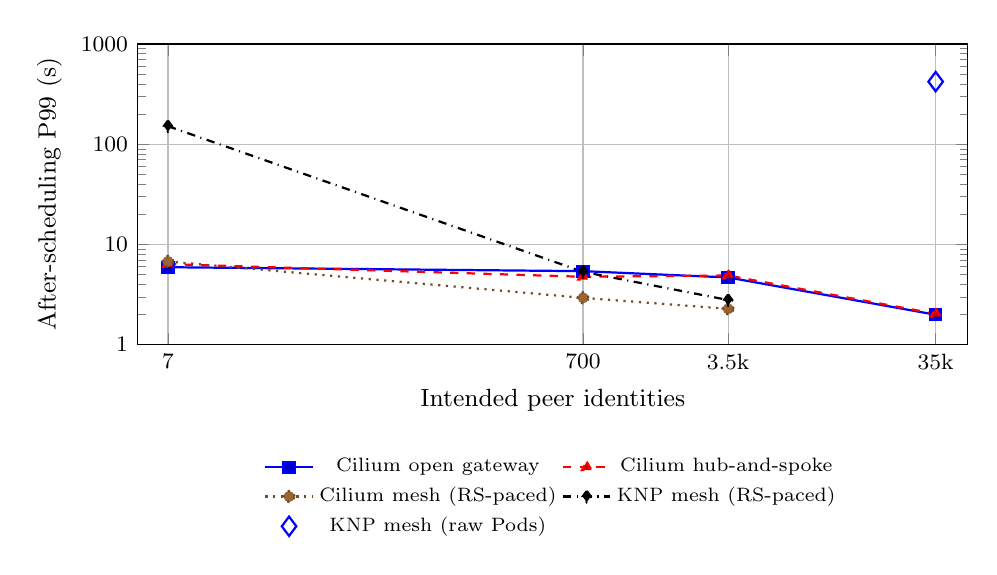
\begin{tikzpicture}
\begin{axis}[width=\linewidth,height=5.4cm,xmode=log,ymode=log,
	xmin=5,xmax=50000,ymin=1,ymax=1000,
	xtick={7,700,3500,35000},xticklabels={7,700,3.5k,35k},
	ytick={1,10,100,1000},yticklabels={1,10,100,1000},
	xlabel={Intended peer identities},ylabel={After-scheduling P99 (s)},
	tick label style={font=\footnotesize},label style={font=\small},
	legend style={font=\scriptsize,draw=none,at={(0.5,-0.34)},anchor=north,legend columns=2},
	grid=major]
\addplot+[mark=square*,thick] coordinates {(7,5.930) (700,5.416) (3500,4.685) (35000,1.990)};
\addlegendentry{Cilium open gateway}
\addplot+[mark=triangle*,dashed,thick] coordinates {(7,6.370) (700,4.759) (3500,4.899) (35000,2.033)};
\addlegendentry{Cilium hub-and-spoke}
\addplot+[mark=*,dotted,thick] coordinates {(7,6.767) (700,2.934) (3500,2.279)};
\addlegendentry{Cilium mesh (RS-paced)}
\addplot+[mark=diamond*,dashdotted,thick] coordinates {(7,151.479) (700,5.331) (3500,2.791)};
\addlegendentry{\sys{} mesh (RS-paced)}
\addplot+[only marks,mark=diamond,mark size=3.5pt,thick] coordinates {(35000,421.410)};
\addlegendentry{\sys{} mesh (raw Pods)}
\end{axis}
\end{tikzpicture}
\end{minipage}\hfill
\begin{minipage}{0.48\textwidth}
\centering
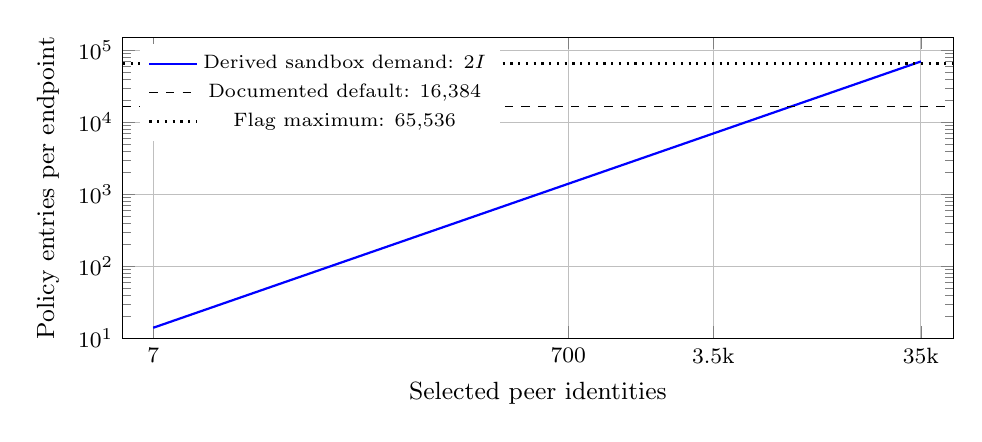
\begin{tikzpicture}
\begin{axis}[width=\linewidth,height=5.4cm,xmode=log,ymode=log,
	xmin=5,xmax=50000,ymin=10,ymax=150000,
	xtick={7,700,3500,35000},xticklabels={7,700,3.5k,35k},
	xlabel={Selected peer identities},ylabel={Policy entries per endpoint},
	tick label style={font=\footnotesize},label style={font=\small},
	legend style={font=\scriptsize,draw=none,at={(0.02,0.98)},anchor=north west},
	grid=major]
\addplot+[mark=none,thick] coordinates {(7,14) (700,1400) (3500,7000) (35000,70000)};
\addlegendentry{Derived sandbox demand: $2I$}
\addplot+[mark=none,dashed,black] coordinates {(5,16384) (50000,16384)};
\addlegendentry{Documented default: 16,384}
\addplot+[mark=none,dotted,black,thick] coordinates {(5,65536) (50000,65536)};
\addlegendentry{Flag maximum: 65,536}
\end{axis}
\end{tikzpicture}
\end{minipage}
\caption{Different meanings of scaling. Left: measured per-run startup
quantiles on a logarithmic axis so that every executed tier is visible;
connecting lines are visual guides, and the raw-Pod point has no
matched Cilium run. Right: conditional permission-state model for eager
per-endpoint compilation. The runner documents
\texttt{--bpf-policy-map-max} as 65,536 on the Cilium cluster, which admits
the unidirectional 35k tiers and excludes the bidirectional mesh at 35k
($2I=70{,}000 > 65{,}536$).}
\label{fig:scaling}
\end{figure*}

These results prevent a simple claim that identity cardinality alone
causes Cilium startup collapse. They do not prove identity-independent
scaling either: the generator changes controller fan-out and burst size
with each tier. Table~\ref{tab:resources} makes the confound visible.
Achieved Phase-1 scheduling throughput is 277--328 Pods/s (median of
per-second samples) for every Cilium tier with 10 or more Pods per ReplicaSet,
and 169--170 Pods/s for the two 35,000-ReplicaSet tiers; cluster-scoped
Pod LIST P99 latency rises from 14--19 s to 28.8 s in the same tiers.
The low post-scheduling P99 at 35,000 identities therefore coincides
with a slower, controller-limited creation stream, which reduces the
burst each node absorbs. One Pod per ReplicaSet is not equivalent to a
few large ReplicaSets at the same object-operation rate. A controlled
identity-turnover test should hold these quantities fixed and
independently vary label sharing and label freshness.

\begin{table}[t]
\centering
\small
\setlength{\tabcolsep}{3pt}
\begin{tabular}{lrrrr}
\toprule
Scenario & Identities & \multicolumn{1}{c}{Pods/s} & \multicolumn{2}{c}{Node CPU (cores)}\\
 & & P50 / P90 & mean & P99\\
\midrule
Gateway & 7 & 284 / 377 & 0.52 & 0.71\\
 & 700 & 317 / 364 & 0.51 & 0.69\\
 & 3,500 & 316 / 372 & 0.54 & 0.69\\
 & 35,000 & 170 / 182 & 0.56 & 0.81\\
\midrule
Spoke & 7 & 0$^{\dagger}$ / 327 & 0.51 & 0.69\\
 & 700 & 323 / 398 & 0.61 & 0.86\\
 & 3,500 & 321 / 373 & 0.54 & 0.67\\
 & 35,000 & 169 / 181 & 0.55 & 0.78\\
\midrule
Cilium Mesh & 7 & 277 / 376 & 0.54 & 0.72\\
 & 700 & 302 / 351 & 0.54 & 0.67\\
 & 3,500 & 328 / 385 & 0.63 & 0.77\\
\midrule
\sys{} Mesh & 7 & 0$^{\dagger}$ / 310 & 0.52 & 0.66\\
 & 700 & 124 / 134 & 0.48 & 0.61\\
 & 3,500 & 103 / 106 & 0.45 & 0.56\\
 & 35,000 (Raw) & 0$^{\dagger}$ / 97$^{\ddagger}$ & 0.66 & 0.86\\
\midrule
Kindnet QPS 500 & $\sim$7 & 233 / 262 & 0.40 & 0.46\\
Kindnet tuned & $\sim$7 & 190 / 225 & 0.63 & 0.79\\
\bottomrule
\end{tabular}
\caption{Recovered Phase-1 scheduling throughput and worker-node CPU
for the runs in Tables~\ref{tab:identity} and~\ref{tab:qps}. CPU is the
harness's instantaneous node query on 4-vCPU workers, aggregated across
nodes over the run; the Kindnet baseline row uses an earlier
rate-based query and is not directly comparable. $^{\dagger}$More than
half of the per-second samples were zero. $^{\ddagger}$Peak 841 Pods/s.
No memory series exists; the six \sys{} agent queries added for the
mesh sweep returned no samples because the deployed Kindnet build does
not expose the agent's metrics endpoint.}
\label{tab:resources}
\end{table}

Worker CPU does not track intended identity count in either family:
Cilium's mean stays within 0.51--0.63 cores and P99 within 0.67--0.86
across tiers and scenarios, and \sys{} Mesh stays within 0.45--0.66 mean
cores (0.56--0.86 P99). This is a whole-node aggregate that includes kubelet,
runtime, and the sandbox workload; it cannot separate the policy agent's share,
and a per-Pod policy-map dump was not collected. What it does exclude
is a CPU explosion at 35,000 identities on the nodes: if Cilium pays
for identity cardinality in these configurations, it does so in the
operator, the API server, or in map capacity, not in visible worker CPU.

The mesh tiers are the only place the two engines meet on the same
generator and policy. For Cilium, post-scheduling medians remain
approximately 1.41--1.42 s across the three executed tiers, while
end-to-end P99s are 33.534, 28.739, and 21.730 s (initial setup plus wait
durations: 192.109, 137.947, and 109.718 s). For \sys{} at 700 and 3,500
identities, post-scheduling latency is 3.273 s P50 / 5.331 s P99 and
2.234 s P50 / 2.791 s P99, and end-to-end P99 is 5.553 s and 2.918 s,
far below Cilium's end-to-end values because \sys{}'s
\texttt{create\_to\_schedule} P99 was 0.4 s and 0.2 s. Two confounds
prevent reading this as an engine comparison. First, the \sys{} runs
achieved 124 and 103 Pods/s median Phase-1 throughput against Cilium's
302 and 328 on the same configured 500 QPS and identical control-plane
settings; each \sys{} node therefore absorbed Pods at well under half
the rate, which by the paper's own argument lowers the per-node burst
and the tail. The cause of the slower creation stream on the Kindnet
cluster is not recorded. Second, each cell is a single trial. What the
matched tiers do support is narrower: under a generator that Cilium
handles at 2.3--2.9 s P99, \sys{} handles 700 and 3,500 identities at
2.8--5.3 s P99 with the gateway-admission gate included, and its worker
CPU does not rise with identity count.

Version matters as much as cardinality. An archived Cilium v1.18.6
attempt at the 700-identity gateway tier, run three hours before the
v1.20.1 sweep on the same day, retains only its generated configuration
and metadata: the harness never produced a startup report. The repository's narrative
records 34,981 Pods Running and 19 stranded in \texttt{Init:0/1} under
default deny, and attributes the outcome to a policy-cache race between
identity allocation and endpoint regeneration tracked as Cilium issue
7515 and resolved in v1.20.0~\cite{cilium7515}. We have not reproduced
that diagnosis from logs. The point for this paper is narrower: the
same generator, at the same tier, produced an admission failure on one
release and a clean 5.4-s P99 on the next. Identity-scaling claims
about eager-materialization systems are release-specific, and a
comparison must pin and report the version it tested.

\subsection{Capacity Exclusion Is Not a Latency Sample}
The mesh experiment producer explicitly excluded the 35,000-identity
tier on Cilium. Its model assigns an entry for each sandbox identity in both
directions at every endpoint. Equation~\ref{eq:materialization} then
gives approximately 70,000 sandbox entries per endpoint, before gateway,
DNS, or other entries. This exceeds the stated 65,536-entry capacity.
The runner lists only the three smaller tiers for Cilium and contains a guard
that skips estimated demands at or above the configured map limit.

This is meaningful design evidence: a system can have low latency
throughout its feasible region and still encounter a state-capacity
boundary. It is not evidence that an executed 35,000-identity mesh on Cilium
experienced insertion failures, packet loss, or a particular latency.
We label it an \emph{analytical exclusion}. The effective
\texttt{--bpf-policy-map-max} on the Cilium cluster is not archived: the
runner reads it from the \texttt{cilium-config} ConfigMap at run time and
falls back to the documented default of 16,384, and its header records
the tested value as 65,536, the flag's maximum~\cite{ciliumagentref}. The
completed runs corroborate the higher value independently. The gateway
policy admits ingress from every sandbox identity, so at 35,000
identities each gateway endpoint needs about 35,000 entries; behind a
16,384-entry map, Pods beyond that count could not pass their
\texttt{wait-for-gateway} gate and would not have reached
\texttt{Running}. All 35,000 did, in both unidirectional 35,000-identity
tiers, so the effective limit was at least 35,000 unless v1.20.1's
identity aggregation applied, which the source restricts to
cluster-, world-, and node-level entity buckets rather than label
selectors. A \texttt{cilium-dbg bpf policy get} dump on one gateway node
would settle the value; none was taken. The agent also exposes an
endpoint-lockdown-on-overflow option~\cite{ciliumagentref}, so an
executed overflow would surface as denied traffic rather than as a
startup latency, which is one more reason the unrun tier has no P99.

Under the benchmark model, 3,500 selected identities and 50 local
endpoints imply approximately 350,000 sandbox policy entries per node.
This is derived demand, not a map dump or a memory measurement.
The contrast with \sys{} is structural: its inspected design does not
require this permission cross-product, so no per-endpoint capacity
excluded its 35,000-identity mesh tier, and that tier completed with
every Pod Running. Its capacity limits lie elsewhere---metadata storage,
conntrack sizing, and userspace decision rate under connection
establishment---and the 421 s tail of that same tier shows that removing
the map bound does not by itself make the tier cheap.

\subsection{An Aborted Direct-Burst Run}
The raw-Pod microsegmentation record documents a different outcome.
An experiment creating Pods directly at the configured 500-QPS tier
aborted with 29,306 Running and 5,694 stranded out of a 35,000-Pod
target. The record attributes the abort to local Cilium REST API
rate limiting during concurrent CNI ADD calls and exhaustion of the
65,280 allocatable cluster-local identities across creation and churn.
It reports the allocator message ``no more available IDs in configured
space.'' No final latency results were generated.

The missing percentile file is not a reason to erase a failed run.
However, the documented diagnosis is not the same as a reconstructed
event timeline. Allocator history, garbage collection, effective limiter
settings, and the underlying logs are needed to separate the two causes
and determine their interaction. Historical allocations can exceed the
live-Pod count, but turnover alone does not imply monotonic consumption
of an unreclaimable identity space.

The allocator namespace here is cluster-level state. It is distinct
from the per-endpoint policy-map capacity used to exclude mesh tier 4.
Likewise, direct Pod bursts differ from ReplicaSet-mediated creation.
The raw-Pod abort supports an admission-failure case study, not an
assertion that every 35,000-identity workload fails or that the unrun
mesh tier has a measurable failure P99.

\subsection{Connection Cost and Correctness}
The available collection measures workload startup and associated
control-plane activity, not the core packet-admission tradeoff. It does
not establish NFQUEUE verdict capacity, established-flow throughput
parity, or isolation through startup and failure. It does bound
first-permitted-connection latency, because the \texttt{wait-for-gateway}
gate of Section~\ref{sec:evaluation} folds one admitted connection into
every \texttt{schedule\_to\_run} sample, but it does not isolate that
component from image pull and container start. A configured mesh
permission does not create all-to-all traffic, and reaching
\texttt{Running} does not test any forbidden peer relationship; the
only negative check is the one-shot smoke test described there.

The only connection-level data point is the repository microbenchmark
summarized in Section~\ref{sec:model}: 2,317 new connections/s through
the queue on one node with sub-millisecond callback medians, and a P99
above 3 s once conntrack was exhausted~\cite{knptesting}. Read against
the startup sweeps, it says that a node absorbing 50 sandboxes at
170--330 Pods/s cluster-wide is nowhere near the queue's connection
limit, and that the limit is reached first by connection-tracking
capacity rather than by the userspace evaluator. It does not say what
happens under sustained denied traffic, whether the P99 is queueing or
conntrack, or how the numbers change with policy count.

The minimum discriminating extension is a small, controlled comparison
of fresh and reused TCP/UDP flows at increasing offered rates, with
permitted and denied traffic kept separate. It should report achieved
connection rate, application-visible P50/P99 setup latency, queued
packets per successful connection, agent CPU, queue drops, and conntrack
occupancy. Repeated trials should include overload, rather than stop
before the queue becomes the bottleneck, and should run once with
fail-open and once fail-closed to measure the bypass window of
Section~\ref{sec:design}. This can test the displaced cost without
repeating a full 720-node sweep.

A companion lifecycle test should establish policy before Pod creation,
then observe runtime metadata delivery and both allowed and forbidden
connectivity from init containers onward. An NRI ablation needs otherwise
identical versions and fairness settings. Policy changes, agent restart,
queue overflow, and IP reuse are required to delimit the safety claim.
These are remaining evaluation requirements, not experiments whose
results this draft assumes.

\subsection{Control-Plane Sensitivity and Limitations}
The July QPS experiments illustrate why startup must be decomposed.
Table~\ref{tab:qps} reports primary saved Cilium and Kindnet baseline
runs. At QPS 500, their post-scheduling P99s are 5.482 s and 57.068 s,
respectively. The archived baseline therefore does not establish a
general startup advantage for the NFQUEUE-based configuration. At
QPS 50 and 100, both families record two JUnit failures. All four are
the same measurement, \texttt{WaitForOldPodsDeleted-Final}, timing out
while 5,024 to 19,999 sandbox Pods from the churn phase were still
terminating; no startup-phase measurement failed. The startup
percentiles in those rows are therefore complete, but the runs did not
finish their teardown within the harness deadline, and Pod deletion
latency at these tiers is itself unmeasured.

\begin{table}[t]
\centering
\small
\begin{tabular}{rrrrr}
\toprule
QPS & \multicolumn{2}{c}{After scheduling P99} & \multicolumn{2}{c}{Total P99}\\
tier & Cilium & Kindnet & Cilium & Kindnet\\
\midrule
$50^{*}$ & 4.065 & 4.833 & 4.089 & 4.855\\
$100^{*}$ & 1.788 & 7.143 & 1.814 & 7.378\\
200 & 1.845 & 59.347 & 2.285 & 59.485\\
500 & 5.482 & 57.068 & 11.160 & 57.629\\
\bottomrule
\end{tabular}
\caption{Archived primary QPS runs; all values are seconds. Asterisks mark
tiers whose only JUnit failures are final-teardown deletion timeouts in
both configurations; startup measurements completed. These are
complete-stack observations, not an isolated NFQUEUE versus eBPF
comparison.}
\label{tab:qps}
\end{table}

The final Kindnet tuning bundle, labeled version 1.0.1 with NRI and
APF exemption, records a post-scheduling P50 of 2.345 s and P99 of
9.718 s. Its total P99 is nevertheless 95.790 s, with a
create-to-schedule P99 of 94.555 s. This juxtaposition is evidence
against interpreting a reduced post-scheduling tail as an automatic
end-to-end speedup. Versions, runtime integration, and API fairness
settings changed together, so the sequence is not a causal NRI ablation.
A separate Cilium QPS-500 repetition records 4.257 s post-scheduling
P99 and 12.404 s total P99; it is retained as a separate trial.

API Priority and Fairness (APF) divides API-server concurrency among
request classes and provides queueing and isolation~\cite{k8sapf}.
Increasing one class's share or exempting it can shift contention to
other components; it does not create storage, CPU, or network capacity.
The API server also mediates most declarative control-plane changes,
including authorization, admission, persistence, and watch delivery.
Its central role makes API latency relevant to network-policy evaluation,
without implying that application packets pass through it.

The collection's limitations affect the conclusions directly. Most
configurations have too few independent trials for statistical claims.
Summary percentiles hide time variation and exclude reconstruction of
individual Pod trajectories. The counts of failed JUnit elements are
not counts of failed Pods. CPU maxima based on instantaneous samples
at the harness's scrape interval are not true peaks. We use these
artifacts to locate the questions the architecture must answer, not
to manufacture a comparative scaling curve from missing measurements.

\subsection{What the Artifacts Still Do Not Contain}
\label{sec:gaps}
The \sys{} mesh sweep closes the largest gap of the earlier draft: a
\sys{} run above seven identities now exists at 700, 3,500, and 35,000.
It does not close the comparison. The harness added six \sys{} agent
queries (verdict rate, processing latency, queue and user drops, CPU,
memory) and a kubelet CNI-latency query, and every one returned no
samples in all four tiers; the repository's own probe script concludes
that the deployed Kindnet build has the agent metrics endpoint disabled.
Table~\ref{tab:gaps} lists what remains. Each row names the missing
evidence, the claim it would support or refute, and the cheapest
experiment that would produce it.

\begin{table}[t]
\centering
\footnotesize
\setlength{\tabcolsep}{4pt}
\newcolumntype{R}[1]{>{\raggedright\arraybackslash}p{#1}}
\begin{tabular}{R{2.35cm}R{2.15cm}R{2.85cm}}
\toprule
Missing evidence & Claim at stake & Cheapest producer\\
\midrule
Agent CPU, memory, verdict rate, latency, drops (all six queries empty) & where displaced work lands; $\lambda_q$, $\mu$, fail-open window & rebuild Kindnet with the metrics server enabled; rerun one tier\\
\addlinespace
Cause of the \sys{} 151 s and 421 s tails & burst behavior of the \sys{} node path & collect init-container \texttt{Latency:} logs and kubelet PLEG/CNI metrics on a sample of nodes\\
\addlinespace
Why \sys{} runs created Pods at 103--124 Pods/s versus Cilium's 302--328 & validity of the matched-tier comparison & compare controller-manager and API-server metrics of the two clusters\\
\addlinespace
A Cilium raw-Pod mesh run or a \sys{} 1-Pod-per-ReplicaSet 35k run & a matched pair at 35,000 identities & one additional run on either cluster\\
\addlinespace
Repeat trials & any statistical statement & rerun tiers 2--3 on both clusters\\
\addlinespace
Policy-map occupancy dump and the effective map-size flag & capacity model of Fig.~\ref{fig:scaling} & \texttt{cilium-dbg bpf policy get} and the ConfigMap on one node\\
\addlinespace
Denied traffic under load & isolation, deny amplification & single-node connection microbenchmark with deny mix, fail-open and fail-closed\\
\addlinespace
NRI on/off with identical binaries & startup-metadata benefit & rerun baseline QPS 500 and tuning bundle 1 with one pinned image\\
\addlinespace
Binary digests and flags per run; logs for both aborts & attribution and causal diagnosis & record in \texttt{cl2-metadata}; retain logs on abort\\
\bottomrule
\end{tabular}
\caption{Evidence still absent from the benchmark and implementation
repositories after the \sys{} mesh sweep.}
\label{tab:gaps}
\end{table}

\section{Related Work}
The closest precedent is reactive virtual switching, not another use
of a kernel packet API. OVS combines userspace classification with
kernel flow caches and discusses the performance consequences of that
architecture~\cite{pfaff2015ovs}. NVP addresses distributed logical
network realization~\cite{koponen2014nvp}; OVN supports stateful
ACLs~\cite{ovnacl}. Our proposed distinction is evaluation of Kubernetes
policy semantics without eager per-endpoint peer materialization,
coupled to local runtime metadata. We do not claim the invention of
userspace miss handling, cached verdicts, or stateful filtering.

Andromeda separates flow-processing paths to reconcile provisioning,
isolation, performance, and feature velocity~\cite{dalton2018andromeda}.
ONCache identifies repeated work across container-overlay layers and
caches invariant results, including filtering, using
eBPF~\cite{oncache2025}. These systems reinforce the importance of
choosing what to cache and when to invalidate it. \sys{} focuses on
the timing of semantic policy work, whereas ONCache accelerates repeated
overlay processing. Its microbenchmark and application evaluations
also illustrate the evidence missing from a startup-only comparison.

KUBEDIRECT identifies API-mediated controller communication as a
serverless scaling bottleneck and develops state management for a
more direct path~\cite{kubedirect2026}. It is relevant to our distinction
between local runtime observation and eventual publication of state,
but NRI-based address discovery does not provide KUBEDIRECT's broader
controller coordination. Role-based micro-segmentation infers endpoint
roles and policies from traffic~\cite{mani2025microsegmentation}; this
addresses policy construction rather than enforcement of a given policy.

Finally, metadata aggregation is established practice. Calico Typha
maintains datastore state, deduplicates events, and distributes updates
to node agents to reduce their individual load on the
datastore~\cite{calicotypha}. The IPTracker direction discussed next
must therefore be evaluated on its representation, caching, and
recovery tradeoffs, not on the novelty of inserting a distribution tier.

The eager-materialization model of Section~\ref{sec:model} is one
representation, not the only kernel-resident one. Open vSwitch's
conjunctive match (\texttt{conj\_id}) lets a rule with $n$ source and
$m$ destination members be installed as $n+m$ flows rather than
$n\times m$~\cite{ovsfields}, and Antrea's OVS pipeline uses exactly
this to compile Kubernetes NetworkPolicy, marking established
connections in conntrack so that only new flows traverse the policy
tables~\cite{antreapipeline}. Calico's Felix compiles selectors into
ipsets referenced by a bounded number of iptables or nftables rules, so
per-endpoint state grows with the number of \emph{rules} rather than
peers~\cite{calicoarch}. Both approaches keep semantic evaluation in
the kernel and avoid the per-peer cross-product by factoring the match;
\sys{} avoids it by moving the match to userspace and caching the
result. A fair capacity comparison must therefore include a
factored-kernel baseline, not only the per-identity expansion that
motivated the mesh-tier exclusion.

\section{Discussion and Future Work}
\subsection{Compact Metadata Distribution with IPTracker}
\label{sec:iptracker}
Avoiding a distributed security-identity allocator does not eliminate
distributed metadata. With $N$ agents each watching all Pod updates,
an update stream of rate $U$ entails approximately $NU$ deliveries
under an all-subscriber model. This is a first-order count, not a
complete performance model; filtering, watch caching, event contents,
and implementation details determine the actual cost.

IPTracker, introduced in the implementation's PR 190, moves full Pod
observation to an intermediate set of distributors and exposes compact
IP-to-Pod records to agents~\cite{iptracker190}. If $R$ distributors
serve $N$ nodes, the policy agents' full Pod subscriptions against the
API server can fall from $N$ to $R$. Other subscriptions remain, and
the distributor-to-agent fan-out does not disappear. In the inspected
client, each agent watches the entire compact-record prefix. This is
not selective subscription to only the peers an agent contacts.

The records are serialized with Protocol Buffers and may be stored
locally in bbolt, with an in-memory LRU in front~\cite{iptrackerbolt}.
Kubernetes can itself use protobuf, so the relevant distinction is
the reduced schema and distribution architecture, not a blanket
JSON-versus-protobuf comparison. The disk store also records revision
metadata for synchronization. A cache miss can consult local storage
rather than perform a per-packet network lookup.

Locality offers a potential memory benefit: a node may communicate
with a small fraction of the cluster's endpoints even when it stores
metadata for all of them. However, a bounded object cache is not
a bound on process or machine memory. bbolt mappings and page cache,
full-sync response buffers, and whole-store listing contribute memory
cost. The present LRU admits updates as well as lookup results, so
metadata churn can evict frequently contacted peers. Store access
under the wrapper's mutex can also couple writes and lookup latency.

Recovery and freshness are equally important. The current full sync
fetches the prefix, clears local state, and inserts records; this
does not establish atomic snapshot replacement or constant-memory
bootstrap. Revision recovery, compaction, reflector failover, disk
failure, and IP reuse must be evaluated before persisted state is
treated as current authorization metadata. Issue 114659 provides
additional motivation for reducing informer memory costs, but it is
not a quantitative demonstration of this implementation's
benefit~\cite{k8s114659}.

The only quantitative data on IPTracker are the single-client
integration-test logs posted with the repository's scalability test
(PR 218)~\cite{iptracker218}. With 10,000 records the server reported
35 MB of Go heap, 643 ms average propagation delay, and a 1 MB client
store. A 40,000-record run at 30,000 writes/s reached 6.6 s propagation
and 174 MB, and the etcd maintainer participating in the thread
observed watch propagation stalling above that size. A 10-million
record run throttled to 1,024 writes/s completed in 9,828 s with 43 ms
average propagation, 24.7 GiB of server heap, and a 1.25 GiB client
store. These are one process on one machine with no packet path, and
the LRU in that test was sized to hold every record, so they bound
neither agent memory under eviction nor the fan-out to hundreds of
clients. They do show that the distribution tier, not the client,
holds the bulk of the state, and that write rate rather than record
count governs propagation delay in the tested range. IPTracker is
implemented future work in this paper's evaluation scope, not a
feature credited with the reported startup results.

\subsection{Testing the Architectural Hypothesis}
The most informative next result is not necessarily a larger cluster.
First, effective software versions, identity counts, map limits,
and the source of each plotted result must be fixed. Existing
lower-tier map dumps could validate the capacity model without
executing a tier already excluded by the harness. Existing failure
logs could establish the allocator and limiter timeline without
reproducing an expensive abort.

Second, workload cardinality and workload freshness should be varied
independently. A matched experiment can retain the same live-Pod count,
generator, placement, offered rate, and policies while alternating
between replacements that reuse label sets and replacements that
introduce new ones. Measuring first permitted communication alongside
startup and actual map occupancy would distinguish distribution and
materialization from unrelated controller delay.

Third, the connection-cost experiment must determine when deferred
evaluation stops being advantageous. If accepted-flow reuse is low,
denied demand is high, or strict revocation repeatedly invalidates
cached decisions, the userspace path may dominate. These outcomes
would delimit the design's useful region, not invalidate the use
of NFQUEUE for every workload. Likewise, a demonstrated capacity
benefit would not establish better packet throughput or immunity
to control-plane overload.

\subsection{Limits of the Present Claim}
The design does not promise unlimited identities, constant total
memory, zero startup delay, or topology-independent resource use.
It avoids one form of eager permission expansion by retaining
semantic interpretation in userspace. This is a useful separation
only if the resulting admission and consistency costs are acceptable.
The \sys{} mesh sweep shows that a tier excluded for Cilium by
per-endpoint capacity completes under \sys{}, and that 700 and 3,500
identities cost \sys{} no more than seven do; it also shows a 151 s tail
under a 5,000-Pod-per-ReplicaSet burst that Cilium absorbs in 6.8 s, at
lower achieved throughput and with one trial per tier. The benefit is
therefore demonstrated for capacity and not yet for admission latency,
and the packet-level boundary remains for the measurements of
Table~\ref{tab:gaps}.

\section{Conclusion}
Network-policy scalability is a joint problem of state representation,
work placement, and synchronization. Fast kernel lookups do not
guarantee cheap workload admission, and a flat latency curve does
not imply unbounded policy capacity. NFQUEUE and conntrack provide
an existing foundation for a different decomposition: interpret
Kubernetes policy when communication is attempted and retain accepted
connection decisions in the kernel. NRI can remove the asynchronous
API round trip from local Pod-address discovery without pretending
to eliminate all distributed-state dependencies.

The archived experiments on 35,000 Pods and 720 workers show both
sides of this trade-off. Completed Cilium sweeps retain low
post-scheduling latency and flat worker CPU within their feasible
region, halve achieved throughput under 35,000 ReplicaSets, exclude the
35,000-identity bidirectional mesh on predicted map capacity, and
stranded 5,694 Pods in one hub-and-spoke raw-Pod burst. The \sys{}
mesh sweep completes that excluded tier with every Pod Running, matches
Cilium within 2.4 s P99 at 700 and 3,500 identities, and records tails
of 151 s and 421 s in its two burst tiers that the artifacts cannot yet
attribute. Because every sandbox gates on a permitted connection to the
gateway, these latencies include first permitted communication across
nodes, which makes them more informative than plain container startup
and also makes the unexplained tails more important. Completing the
comparison requires the measurements of Table~\ref{tab:gaps}, starting
with an agent build that exposes its metrics and a repeat of the
matched tiers.

\clearpage
\bibliographystyle{plain}
\bibliography{references}

\clearpage
\appendix
\section{Evidence Provenance}
\label{sec:provenance}
This appendix is an internal provenance guide for the non-submission
exercise. Paths are relative to the benchmark repository unless
stated otherwise. It is not anonymized publication material.

\paragraph{Archived numeric results.}
The extractor is \path{submission/analyze.mjs}; the current extraction
(covering all 66 benchmark runs and 59 startup reports) is recorded in
\path{submission/upstream/inventory.json},
\path{submission/upstream/startup.csv}, and
\path{submission/upstream/extracted-results.md}. Run names do not
independently establish tested software versions.

Table~\ref{tab:identity} and the measured panel of
Figure~\ref{fig:scaling} use reports beneath
\path{artifacts_pods/cilium/identity-sweep/},
\path{artifacts_pods/cilium/microsegmentation/},
\path{artifacts_pods/cilium/mesh-sweep/}, and
\path{artifacts_pods/kindnet/mesh-sweep/}. The Cilium mesh reports are in
\path{tier1-7-identities-5000ppr},
\path{tier2-700-identities-50ppr}, and
\path{tier3-3500-identities-10ppr}. Their sibling
\path{*-initial} directories contain hook logs, not startup reports.
The \sys{} (Kindnet) bidirectional mesh reports are in
\path{artifacts_pods/kindnet/mesh-sweep/tier1-7-identities-5000ppr},
\path{tier2-700-identities-50ppr},
\path{tier3-3500-identities-10ppr}, and
\path{tier4-35000-identities-rawpods}. Their
\path{generatedConfig_agentic-sandboxes.yaml} files set
\texttt{SandboxPeerMode: mesh}; the Cilium raw-Pod directory under
\path{microsegmentation/} does not, which is why the two raw-Pod runs
are not a matched pair. The tier-4 \path{junit.xml} records the two
startup-SLO failures. The \path{GenericPrometheusQuery Kube Network
Policies *} and \path{... Kubelet CNI Plugin Operations Latency} files in
all four tiers contain \texttt{"dataItems": null}; the queries are
defined in \path{manifests/agentic-sandbox/measurements/knp-measurements.yaml}
and \path{scripts/query-kindnet-metrics.sh} records that the Kindnet
build exposes no metrics port.

\paragraph{Enforcement gate.}
The \texttt{wait-for-gateway} init container is defined in
\path{manifests/agentic-sandbox/manifests/sandbox-pod.yaml} and
\path{sandbox-replicaset.yaml}; the policies that make the gate a
permitted-connection test are \path{global-sandbox-policy.yaml} (sandbox
egress to \texttt{group: gateway}) and \path{gateway-policy.yaml}
(gateway ingress from \texttt{group: sandbox}), with
\path{default-deny-policy.yaml} applied in every archived run
(\texttt{ApplyDefaultDenyPolicy: true}). The one-shot negative check is
\path{scripts/verify-netpol.sh}; no output of it is archived.

Table~\ref{tab:qps} uses the primary runs under
\path{artifacts_pods/cilium/qps-*}, including
\path{qps-500/verified-run}, and
\path{artifacts_pods/kindnet/baseline-sweep/qps-*}.
The separate Cilium trial is in \path{qps-500/repeat-run}.
The final Kindnet tuning bundle is under
\path{artifacts_pods/kindnet/500qps-optimizations/5-v1.0.1-plus-nri-plus-apf-exempt/}.
The teardown-timeout diagnosis of the asterisked rows is from the
\path{junit.xml} files in the QPS 50 and 100 directories of both
families.

\paragraph{Recovered throughput, CPU, and API latency.}
Table~\ref{tab:resources} reads \path{Phase1SchedulingThroughput_*.json}
(\texttt{perc50}, \texttt{perc90}) and
\path{GenericPrometheusQuery Worker Node CPU Utilization_*.json}
(\texttt{mean\_}, \texttt{p99\_instantaneous\_node\_cpu\_cores}) in
each run directory; the Kindnet baseline uses \texttt{mean\_node} and
\texttt{p99\_node} from an earlier query. Pod LIST latency is the
cluster-scoped \texttt{pods/LIST} row of
\path{APIResponsivenessPrometheus_simple_*.json}. The hub-and-spoke
rows come from \path{artifacts_pods/cilium/microsegmentation/tier*}.
The extraction is reproducible with \path{submission/analyze.mjs};
no value was transcribed from the repository's Markdown summary.

\paragraph{Archived v1.18.6 attempt.}
\path{artifacts_pods/archive/v1.18.6-identity-runs/} holds a complete
7-identity run and a 700-identity directory containing only
\path{cl2-metadata.json} and the generated configuration. The
34,981/19 counts and the issue-7515 attribution are from
\path{benchmark_results.md}, not from artifacts.

\paragraph{Outcome records and capacity model.}
Revision \texttt{0442dce} adds
\path{artifacts_pods/cilium/microsegmentation/tier4-35000-identities-rawpods/README.md},
the source of the 29,306/5,694 completion counts and stated diagnosis.
Revision \texttt{f998224} adds
\path{artifacts_pods/cilium/mesh-sweep/README.md}, documenting the
unexecuted Cilium mesh tier. Revision \texttt{5b152f2} adds
\path{artifacts_pods/kindnet/mesh-sweep/}: three ReplicaSet-paced
\sys{} tiers matched to the Cilium mesh generator and one raw-Pod tier.
Its README's ``under 50 seconds'' scheduling statement is contradicted
by the archived \texttt{create\_to\_schedule} P99 of 106.7 s, and its
``0 CNI errors'' has no backing metric; neither is used here.
The model and exclusion are cross-checked against
\path{scripts/run-mesh-sweep.sh} and
\path{manifests/policy-scenarios/scenario-c-mesh-bidirectional.yaml}.
The 65,536 map limit is documented only in the runner's header comment;
the ConfigMap it reads at run time is not archived.

\paragraph{Original charts.}
The input figure \path{figures/fig2_identity_cardinality_sweep.png}
mixes measured quantiles, unmatched Kindnet tier values, and a failure
bar. The separate \path{figures/fig2_topological_scaling_p99.png}
contains a 94.3-second overflow value and a kernel-set description of
\sys{} that the audited evidence does not support. Both originals
are preserved; neither is reproduced as a verified result here.
Figure~\ref{fig:scaling} is typeset directly from the audited quantiles
and the explicitly conditional capacity model.

\paragraph{Implementation.}
Paths in the companion kube-network-policies repository are
\path{pkg/dataplane/controller.go} (queue configuration, bypass flag,
postrouting and input chains), \path{pkg/cmd/cmd.go}
(\texttt{--fail-open} default), \path{pkg/networkpolicy/networkpolicy.go}
(\texttt{nil}-peer selector semantics, managed-IP set),
\path{plugins/iptracker/iptracker_networkpolicy.go} (divert-all),
\path{pkg/podinfo/nri/resolver.go}, \path{pkg/ipcache/{client,bbolt,lru}.go},
and \path{docs/testing/README.md} with its two PNG charts, inspected at
\texttt{9984dcd}. Benchmark-side deployment facts are from
\path{manifests/kube-network-policies-install.yaml} and
\path{scripts/create-netpol.sh}. Source behavior has not been equated
to the benchmark binaries. \path{submission/evidence-audit.md} records
the claim-level audit, and \path{submission/author-guide.md}
provides the prioritized remaining checks.
\end{document}
